%\documentclass[11pt,a4paper,openright]{report}
\documentclass[project,twoside]{iitbreport}

\usepackage[toc,page]{appendix}
\usepackage{titlesec}
\titlespacing\section{0pt}{12pt plus 4pt minus 2pt}{0pt plus 2pt minus 2pt}
\titlespacing\subsection{0pt}{12pt plus 4pt minus 2pt}{0pt plus 2pt minus 2pt}
\titlespacing\subsubsection{0pt}{12pt plus 4pt minus 2pt}{0pt plus 2pt minus 2pt}
%\titlespacing\subsection{0pt}{12pt plus 4pt minus 2pt}{0pt plus 2pt minus 2pt}

%% Selectively comment out sections that you want to be left out but
%% maintaining the page numbers and other \ref
%\includeonly{%
%  introduction,
%  ref,
%  conclusion
%}

%%% Some commonly used packages (make sure your LaTeX installation
%%% contains these packages, if not ask your senior to help installing
%%% the packages)
%\usepackage{pdfpages}
\usepackage{mathtools}
\usepackage{program}
\usepackage{algorithm}
\usepackage[noend]{algpseudocode}
\usepackage{booktabs}
\usepackage{fixltx2e}
\usepackage{url}
\usepackage{pbox}
\usepackage{graphicx}
\usepackage[T1]{fontenc}
\usepackage{enumitem}
\usepackage{amsmath}
%\usepackage{enumerate} %lower-case roman numerals in enumerate lists
\usepackage{multirow} %for table
\usepackage{hhline} %for table
\usepackage{subcaption} %for subcaption in sub-figures
\setlist{nosep}
\graphicspath{{images/}}
\newcommand{\dud}[1]{\underline{#1}}
%python
\usepackage{listings}
\usepackage{color}

\newcommand{\mle}{$ \le $}
\newcommand{\marr}{$ \rightarrow $}

\definecolor{codegreen}{rgb}{0,0.6,0}
\definecolor{codegray}{rgb}{0.5,0.5,0.5}
\definecolor{codepurple}{rgb}{0.58,0,0.82}
\definecolor{backcolour}{rgb}{0.95,0.95,0.92}

\lstdefinestyle{mystyle}{
	backgroundcolor=\color{backcolour},   
	commentstyle=\color{codegreen},
	keywordstyle=\color{magenta},
	numberstyle=\tiny\color{codegray},
	stringstyle=\color{codepurple},
	basicstyle=\footnotesize,
	breakatwhitespace=false,         
	breaklines=true,                 
	captionpos=b,                    
	keepspaces=true,                 
	numbers=left,                    
	numbersep=5pt,                  
	showspaces=false,                
	showstringspaces=false,
	showtabs=false,                  
	tabsize=2
}

\lstset{style=mystyle}
%python2 
% Default fixed font does not support bold face
\DeclareFixedFont{\ttb}{T1}{txtt}{bx}{n}{12} % for bold
\DeclareFixedFont{\ttm}{T1}{txtt}{m}{n}{12}  % for normal

% Custom colors
%\usepackage{color}
\definecolor{deepblue}{rgb}{0,0,0.5}
\definecolor{deepred}{rgb}{0.6,0,0}
\definecolor{deepgreen}{rgb}{0,0.5,0}

%\usepackage{listings}
% Python style for highlighting
\newcommand\pythonstyle{\lstset{
		language=Python,
		basicstyle=\ttm,
		otherkeywords={self,if,while,log},             % Add keywords here
		keywordstyle=\ttb\color{deepblue},
		emph={MyClass,__init__},          % Custom highlighting
		emphstyle=\ttb\color{deepred},    % Custom highlighting style
		stringstyle=\color{deepgreen},
		frame=tb,                         % Any extra options here
		showstringspaces=false            % 
	}}
%endpython
%\renewcommand{\chaptername}{}
\usepackage{titlesec}

\begin{document}
\title{Certification of Python Programs on the Basis of Static Information Flow Analysis}
\author{{\href{http://www.cse.iitb.ac.in/~kush/}{Abhishek Pratap Singh}}\\
	143050077\\
	\vspace{0.5cm} 
	\normalfont \textit{ \centerline{under the guidance of}}
	\vspace{1.0cm} 
	\newline
	{\textbf{Prof. R K Shyamsundar}}}
\degree{Master of Technology}
\dept{\href{http://www.cse.iitb.ac.in/}{Department of Computer Science and Engineering}}
\monthyear{July, 2016}

%\makecoverpage
\maketitle

\begin{abstract}
	In this thesis, we present our work on secure information flow analysis of python programs.
	We have built a platform that takes source code and labels of all objects used in python program as input for static
	analysis of information flow throughout the program. We started with Denning's lattice model [1]
	for verification of secure information flow. In this model, every object is associated with its
	security class. To prevent unauthorized leak of information, the flow of information should be
	in one way -- from less secure to more secure class. A lattice represents such information
	model very well, the upward direction in lattice represents secure information flow. Verification of
	information flow only on the basis of security class is not sufficient to certify the security of system, there is a need to consider the process, user or subject that executes the code. Use of Reader Writer Flow model \cite{denning} with subjects makes it possible to do secure
	information flow analysis. We have developed four type of constraint generators C1, C2, C3 and C4 each implementing different approach. Constraint generator C1 considers fixed label and PC reset(PC reset denotes PC is not retaining information out of scope), C2 considers fixed label and monotonic PC (monotonic PC never lose information), C3 considers dynamic label and PC reset and finally the constraint generator C4 considers dynamic label and monotonic PC. Constraint resolver takes these constraints and RWFM labels [2] for each
	object defined by the user as input and provides answers to various queries related to information
	flow security.The report describes, the approach, implementation and case study done so far.
\end{abstract}

\renewcommand{\abstractname}{\LARGE Acknowledgements}


%\clearpage
\pagenumbering{roman}
\addtocontents{toc}{\vskip-40pt}
\let\cleardoublepage\clearpage
\tableofcontents
\listoffigures
%\listoftables
\lstlistoflistings
\newpage
%\cleardoublepage
%\clearpage
\let\cleardoublepage\clearpage
\setcounter{page}{1}
\pagenumbering{arabic}


\chapter{Introduction}


This document contains commonly used essential templates to write a
\LaTeX\ document. This document is to be used along with the files and
folders provided. Writing a \LaTeX\ document is very simple.  Often
students need only very simple constructs.  This document shows
certain essential features that almost all technical report writing
requires. Please consult the PDF file for the output of the document,
and then look at the corresponding \LaTeX\ file to reproduce it.  The
document illustrates the following constructs
\begin{itemize}
\item Unnumbered and Numbered Lists
\item Equations
\item Defining short macros for frequently used symbols
\item Bibliography
\item Figures
\item Tables
\end{itemize}

The normal procedure for compiling a \LaTeX\ document that contains
bibliographic entries is to follow the following steps
\begin{enumerate}
\item \verb|pdflatex mainrep|
\item \verb|bibtex mainrep|
\item \verb|pdflatex mainrep|
\item \verb|pdflatex mainrep|
\end{enumerate}
In the above example \verb|mainrep| is the main \LaTeX\ file.


\section{First section of this chapter}

This is the first chapter, which resides in a directory (folder)
intro. Each chapter can contain \verb|section|, \verb|subsection|
and so on.

\subsection{Equations and Math symbols}


Equations should be set in a separate mode.  For details on getting
various types of aligned equations, consult the \AmS-\LaTeX\
documentation \verb|amsldoc.pdf|. Simple equations are set as
\begin{equation}
\label{eq:sinx}
\int \mathrm{d}x \; \cos x =  \sin x
\end{equation}
Equation~\eqref{eq:sinx} is the integral of the cosine
function. Mathematical symbols must always be put inside \verb|$$|,
when they appear outside a math environment (such as \verb|equation|,
\verb|align|, \verb|gather|, etc).  The symbol ``ex'' must be written as
$x$ and not as x.  

Another commonly used construct for equations is the \verb|align|
environment to align several equations along a vertical line. It is
usually the $=$ sign across which the alignment is done.  The
point of alignment for each equation is specified using the ampersand symbol 
\begin{align}
a &= b  \\
a + e + f + g & = m + n + z \\
x + 2 & = x^{3} + 3 x^{2} + 2 x + 5
\end{align}

\subsection{Commonly used Symbols}
For mathematical symbols it is very convenient to define frequently
used symbols as a short macro. For example if you are to be using the
symbol $\eta_{\mathrm{s}}$ frequently it is convenient to define it in
as:\\
\verb|\newcommand{\etas}{\ensuremath{\eta_{\mathrm{s}}}}| \\
in the preamble and to simply refer it to in the text as \etas\ or in
a mathematical equation as $\etas = \eta \, ( 1 + \phi)$.

%%% Local Variables: 
%%% mode: latex
%%% TeX-master: "../mainrep"
%%% End: 

\chapter{Background}
\label{ch:bg}       
\subsection{Bell Lapadula security model \cite{lapadula}}
This model defines four senstivity labels "Top secret", "secret", "classified", and "Public" each object must be labled from one of these labels. This model uses mandetory access control , mandetory denotes that they can not be changed. System contains subjects (user) , labeled objects, state machine with a set of states it allowed to go. Model preserves security of information in transitions of one state to another. Introduces (i) *(star) prperty: No Write-Down (NWD), it prevents subjects from higher label to write in to objects of lower label, this stops leak of information. (ii) simple security property: No Read Up (NRU), it prevents subjects from lower label to read from objects from higher label. A access matrix of subject and object is used to define permissions for subjects to use objects. This model is based on confidentiality of information.
\subsection{Biba Security Model \cite{biba}}  
This model ensures integrity of data. To maintain integrity of data it ensures three things (a) Prevention of modification from unathorized user. (b) Prevention of unathorized modification from authorized user. Bia model defines integrity classes and rules to preserve integrity of data. The simple integrity rule says that subjects can not read objects of lower label of integrity (No read down). The *(star) integrity rules says that subjects can not write into objects of higher label(No write up). These rules are in contrast with Bell Lapadula model because Biba model considers integrity of information instead of confidentiality. Here labels denotes degree of trust. Lowest label is not reliable so it is not allowed to write to others similarly highest label is not allowed to read from others otherwise it can be corrupted by unreliable information.
\subsection{Denning's Lattice model \cite{denning}}
This model is based on Lattice model. There is set of security classes each denotes disjoint set of information, unlike previous models it gives facility to perform operation on two security class labels, operations are lub denoted by $\oplus$ and glb denoted by $\otimes$. Both operation helps to calculate security label of an expression involving many objects from different security classes. To preserve security in information flow there is a basic rule: if information flowing from x to y (x\marr y) then for secure information flow constraint \dud{x}$\le$\dud{y} must satisfy, \dud{x} denotes security class of x. So all information flow heading upward in lattice diagram are secure.  
\subsection{Reader Writer Flow Model \cite{rwfm}} 
---



\chapter{Secure Information Flow Analysis of Python Programs}
There have been many studies on information flow control and all of them share some basic properties like information flow should be from less secure entity to more secure entity. Denning's book \cite{denning} has a chapter on information flow control, this chapter describes lattice model for information flow \cite{lattice}, this makes it easy to track information flow in a program using transitivity property. Analysis has been done on basic operations which involve information flow like assignment operation (explicit flow) based on data flow, conditional operations like if else, while etc. (implicit flows) based on control flow, information flow through covert channel based on traps and exception in programs. Here are some basic rules given in \cite{denning}, (arrow $\rightarrow$ denotes information flow).  
\begin{itemize}
	\item x = y : y $\rightarrow$ x
	\item if e then x = y : e $\rightarrow$ x
	\item while w {if e then{ x = y} w =false } : w $\oplus$ e $\rightarrow$ x
	\item infinite loop: while w {}; x = y :- w $\rightarrow$ x etc.   
\end{itemize}
Chen et al. \cite{hybrid}(published in 2014) presented work on python byte-code and claimed that there was no work related to python at that time. They implemented information flow checker for python byte-code using static and dynamic analysis but their main focus is on information flow policies related to objects. Kumar et al. \cite{rwfm} introduce a new model to work with subjects and my work will be focused on this. Conti et al. \cite{taint} provide library support in python for information flow analysis in explicit flows only.
Data Security can be achieved using information flow policies. Execution of any action
like copying of file, read operation on file or memory, write operation on file or memory, execution of statement etc may cause flow of information. Usually, information revealed that was
unknown before execution of statement termed as information flow otherwise if it was known already then there will be no information flow. This thesis focuses on information flow between
variables used in a python program irrespective of the amount of information flowing. There are two kinds of information flow among variables:\\
\begin{enumerate}
	\item{\textbf{Explicit Information Flow}}\\
	\begin{lstlisting}[language=Python, caption=Python example]
	x = y
	x = math.log(y)\end{lstlisting}
	these assignment operations are example of explicit flow because information related to variable y is flowing into x using data dependency in both cases.
	\item{\textbf{Implicit Information Flow}}\\
	\begin{lstlisting}[language=Python, caption=Python example]
	if y == 1:
	x = 1
	\end{lstlisting}
	\pagebreak
	\begin{lstlisting}[language=Python, caption=Python example, label=lst:whilecode]
	while y < z:
	x = 1
	y += 1\end{lstlisting}
	in these examples value of x after execution of statements depends on the control path
	taken by the program, variable y and z used in choosing between two control path in while
	program, this involvement of y and z in making decision reduce the uncertainty of variables
	y and z. Whether y < z or y > z can be observed with help of final value of x after execution of given code in listing \ref{lst:whilecode} . So there is indirect implicit flow from y to x in the first example and implicit flow from y
	and z to x in the second example\cite{denning}.\\~\\
	\begin{lstlisting}[language=Python, caption=Python example, label=lst:infwhile]
	x = 0
	while y == 1:
	pass
	x = 1\end{lstlisting}
	Here assignment operation on x in Listing \ref{lst:infwhile} is outside of while body but still information flowing from y to x because execution of x = 1 statement depends on termination of while loop, so you can know value of y by checking the value of x after execution of program, for example if value of x is 1 and program terminated then y must be other than 1, if while loop goes in infinite loop then y must be 1.
	
	The first chapter describes python program certification with the help of Denning's Lattice Model. The lowest security class in this lattice assumed is Low everyone can read information from this class, the highest class in the lattice is High, 
	information from all security classes can flow into it but no information can flow from this class to others.
	For Example certification of python code in Listing \ref{lst:lattice} needs to follow Denning's lattice and constraints written in figure \ref{fig:lattice}, security class of variable var is denoted by \dud{var}.  
	\begin{lstlisting}[language=Python,caption={Python example}, label={lst:lattice}]
	x = 0
	z = 1
	y = 0
	if x :
	while z :
	y = 1\end{lstlisting}
	\begin{figure*}[h]
		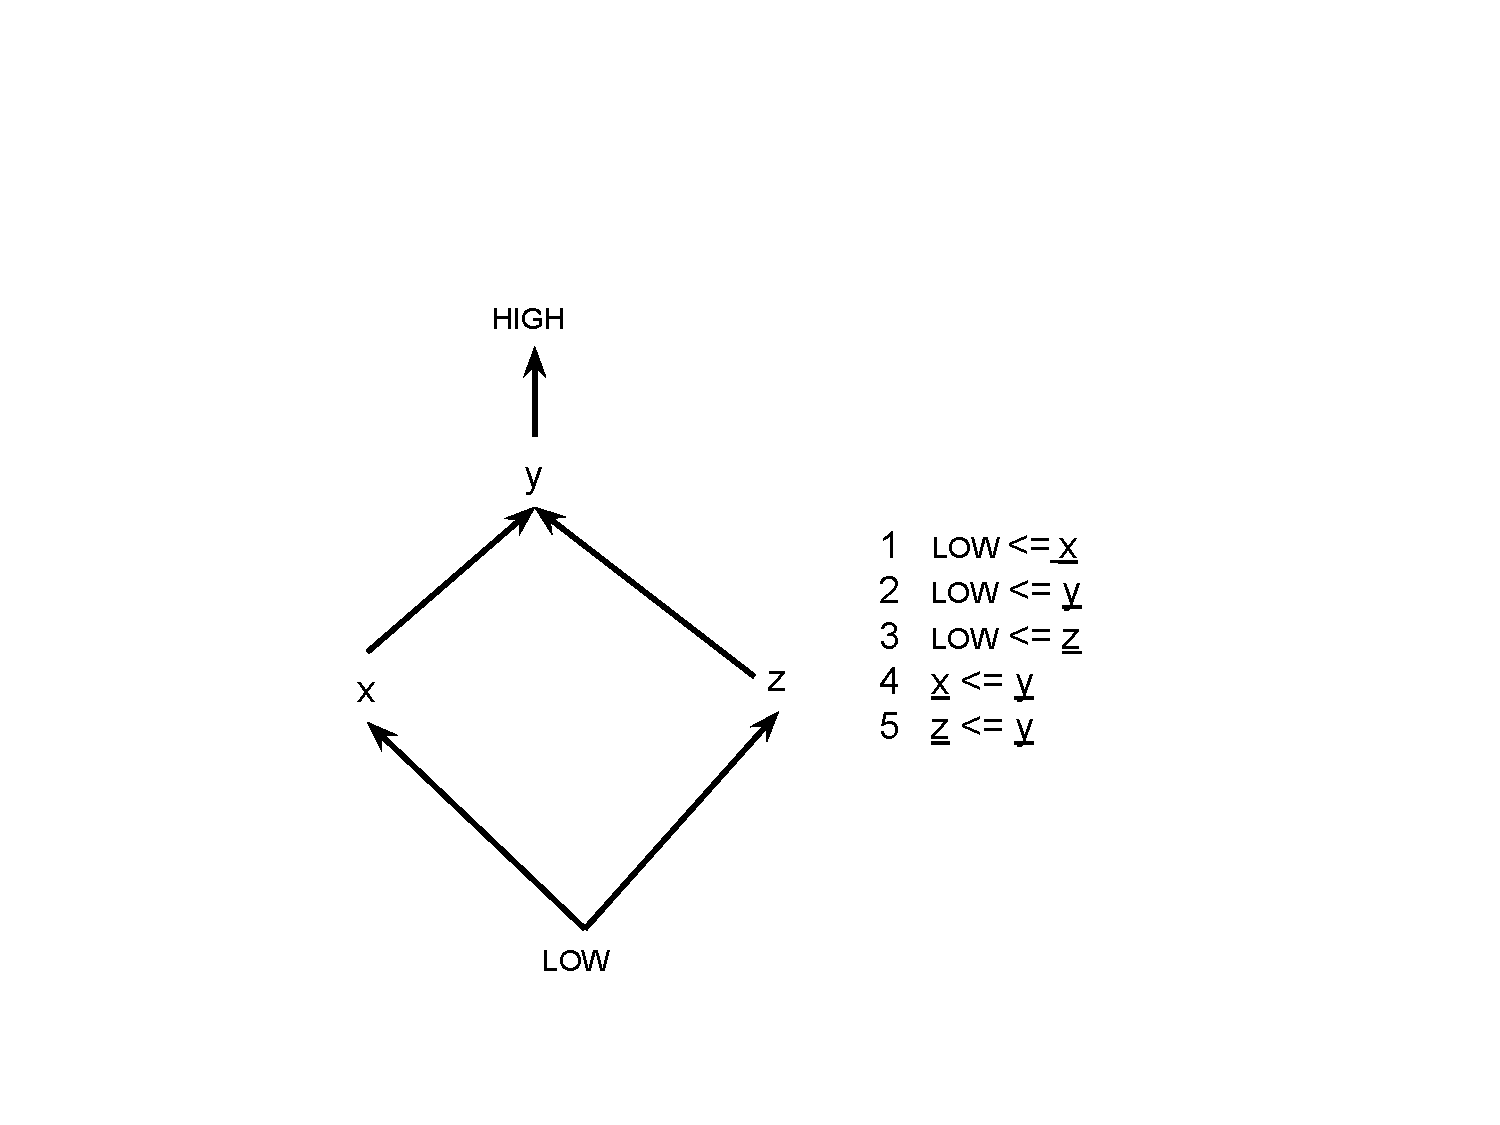
\includegraphics[width=0.6\textwidth]{lattice}
		\centering
		\caption{Lattice of Listing \ref{lst:lattice}}
		\label{fig:lattice}
	\end{figure*}
	Chapter \ref{ch:caseStudy} describes information flow by nonterminating while loop and how to certify program in such situation.
	Chapter \ref{ch:caseStudy} describes how information flows among thread in the multi-threaded program using semaphore.
	Chapter \ref{ch:constgen} presents a new approach to certifying a program using more sophisticated labels (RWFM label)
	and it also considers subjects for certification of the program.	
\end{enumerate}     


\chapter{Approach to certify Python Programs}
\label{ch:certify}
\subsection{ Category 1 constraint Generator : PC reset and fixed labels.}
\label{ch:c1}
This chapter describes working of first algorithm for constraint generation. All four algorithms are different because of different combination of PC label management scheme and  use of dynamic labels. In this algorithm we are using fixed label. Fixed label denotes that label will not change throughout the program. PC reset denotes that after completion of scope of a particular conditional/iteration body PC reset back to the PC just before the execution of conditional/iteration statement. PC monotonic denotes a scheme in which PC label never lose any information once it acquires, it just grows monotonically. This algorithm is able to capture basic information flows within a program, so this algorithm will certify a large number of programs as secure. Program certified secure by this algorithm does not mean that its fully secure, it certifies secure because of the limitation in detection of information flows in program. Some information flows which are not captured by this algorithm may violate information security.\\
\subsection{Working}
All four algorithm shares same basic structure for parsing input program. Dynamic analysis can not process all branches in a one go but static analysis process all branches in one run. Algorithms generates constraints for all possible control branches in program.  PC keeps track of variables used in conditional statement and iteration statement. Assignment operation are responsible for information flows so at each occurrence of assignment operation constraints generated with the help of PC label.
\section{Constraint Rules}
\begin{enumerate}
	\item < x := e > generate constraint [$\lambda(e)\oplus\lambda(PC)\le\lambda(x)$] and update PC label\\ $\lambda(PC) = \lambda(e)\oplus\lambda(PC)$ 
	\item < x := e > generate constraint [$\lambda(e)\oplus\lambda(PC)\le\lambda(x)$] and update PC label\\ $\lambda(PC) = \lambda(e)\oplus\lambda(PC)$ 
	\item < if e then c1 else c2>  $\forall  x \in ( modified\_global(\hspace{0.2cm} c1 \hspace{0.2cm}and \hspace{0.2cm} c2) \cup \{PC\} )$ generate constraints [$\lambda(e)\oplus\lambda(PC)\le\lambda(x)$] and update PC label $\lambda(PC) = \lambda(e)\oplus\lambda(PC)$
	
	\item < while e do c > $\forall  x \in ( modified\_global(c) \cup \{PC\} )$ generate constraints [$\lambda(e)\oplus\lambda(PC)\le\lambda(x)$] and update PC label $\lambda(PC) = \lambda(e)\oplus\lambda(PC)$
\end{enumerate}

\begin{figure}
	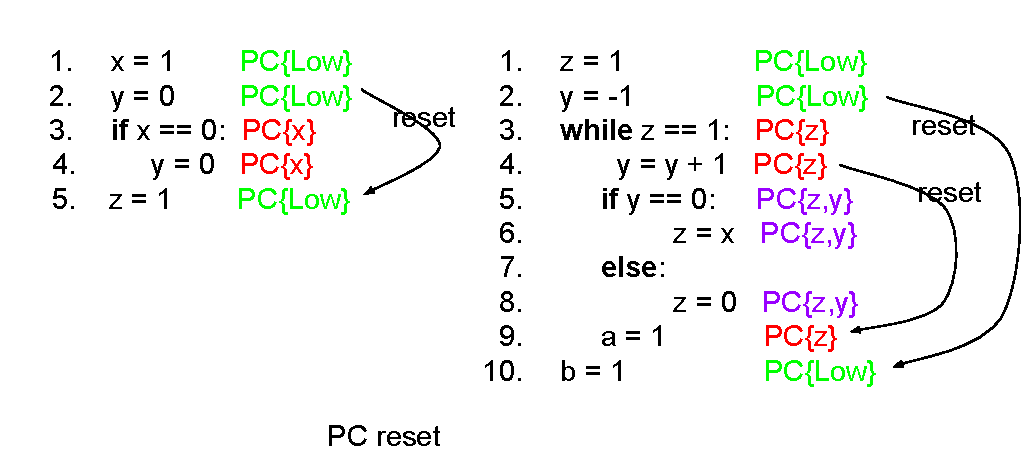
\includegraphics[width=1\textwidth]{PC_reset.pdf}
	\centering
	\caption{Example for PC reset}
	\label{fig:pcreset}
\end{figure}
\begin{figure}
	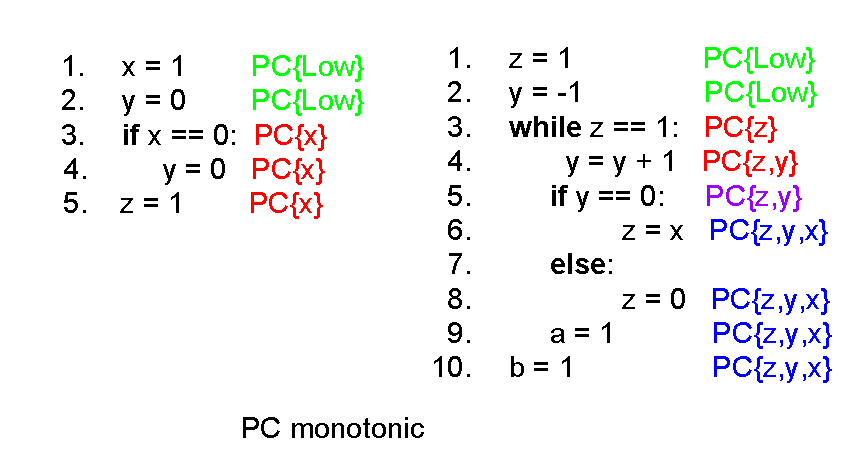
\includegraphics[width=1\textwidth]{PC_monotonic.pdf}
	\centering
	\caption{Example for PC monotonic}
	\label{fig:pcreset}
\end{figure}
\subsection{Key Idea}
Direct information flow happens because of copying or assigning values. Implicit information flow happens because of control dependency, this algorithm focuses on information flow from variables used in condition statement of if else(conditional)
and while(iteration) to all variables modified in the body of iteration or conditional.
\begin{lstlisting}[language=Python,caption={Python example}, label={lst:p1copy1}]
def(x,y):     #copy x to y
y = 0
z = 0
if x == 0:    # implicit flow x -> z PC{x}
z = 1
if z == 0:    # implicit flow z-> y PC{z}
y = 1
p = q         # direct flow q -> p PC{q}
\end{lstlisting}
Constraints generated by this algorithm for listing \ref{lst:p1copy1} are given below. 
\begin{itemize}
	\item x <= z
	\item z <= y
\end{itemize}
\section{Limitations}
For listing \ref{lst:p1copy1} this algorithm is able to capture all information flows, but in more complex programs it may declare falsely a program secure.
\begin{lstlisting}[language=Python, caption=Python version of copy5 example in \cite{denning}. goal: information flow from x to y, label={lst:p1copy5} ]
#Procedure copy5
y = 0
while x==0 :
pass
y = 1
\end{lstlisting}
For listing \ref{lst:p1copy5} this algorithm generated only one constraint Low <= y, that shows this algorithm will certify listing \ref{lst:p1copy5} secure always irrespective of information flow x to y is secure or not. All these limitation in capturing information flow raised because of PC label management in this algorithm is only focus on local information flow. Next algorithm will try to remove these limitation using monotonic PC label management. Appendix A shows the implementation of this algorithm.
\begin{lstlisting}[language=Python, caption=Python version of dynamic label example in \cite{denning}. goal: information flow from x to y, label={lst:p1dynamic} ]
def fun(x, y, z):
a = x
y = a
a = z
fun(x, y, z)
\end{lstlisting}
Another limitation of this algorithm is related to use of fixed label. In listing \ref{lst:p1dynamic} this algorithm detect false information flow z to y. Category 3 uses both dynamic and fixed label to remove this limitation.
\section{Category 2 constraints : PC monotonic and fixed labels.}
This chapter describes working of category 2 constraint generator. This algorithm is a improved version of previous category 1 algorithm. This algorithm using monotonic PC label instead of PC reset. By using monotonic PC this algorithm is able to detect additional information flows in program.
\subsection{Working}
rules
\subsection{Key Idea}
This analysis extension of previous algorithm, non terminating loops
create a control dependency between variables used in condition of loop and
the rest of the code where control can go subsequently on termination of loop,
because of this behavior of non terminating loop PC storing all the dependencies.

\subsection{Limitations}  
In static analysis if constraint resolver ignores the order of generated constraints then it may show some additional false information flow in program, this is responsible for overhead and imprecision in certification process. Use of dynamic label solves this problem easily on the cost of more complex analysis.
\begin{lstlisting}[language=Python, caption=Python version of dynamic label example in \cite{denning}. goal: information flow from x to y, label={lst:p2dynamic} ]
def fun(x, y, z):
a = x
y = a
a = z
fun(x, y, z)
\end{lstlisting}
constraints generated for listing \ref{lst:p2dynamic} are given below:
\begin{itemize}
	\item x <= a
	\item a + x <= y
	\item a + x + z <= a
\end{itemize}
these constraints shows that there is information flow z to y ( using a <= y and z <= a) but in program there is no such flow exist. Because of such information flow constraint resolver may certify a secure program as not secure and it also create extra overhead on resolver. This example shows flaw in approach of using fixed label everywhere. Next algorithm will try to remove this limitation.
\section{Category 3 constraints : PC reset and dynamic labels.}
\label{ch:c3}
This chapter describes category 3 constraint generator. This algorithm introduces use of dynamic label. Global variable are using fixed label and all local variables are assigned dynamic label. Information can flow outside only because of modification of global variable, modification of local variable doe not cause information because information remains in program itself.   
\subsection{Constraint Rules}
\begin{itemize}
	\item < x := e > generate constraint [$\lambda(e)\oplus\lambda(PC)\le\lambda(x)$] and update PC label\\ $\lambda(PC) = \lambda(e)\oplus\lambda(PC)$ 
	\item < if e then c1 else c2> \begin{enumerate}
		\item $\forall  x \in ( modified\_global(\hspace{0.2cm} c1 \hspace{0.2cm}and \hspace{0.2cm} c2) \cup \{PC\} )$ generate constraints [$\lambda(e)\oplus\lambda(PC)\le\lambda(x)$] and update PC label $\lambda(PC) = \lambda(e)\oplus\lambda(PC)$
		\item $\forall x \in ( modified\_local(\hspace{0.2cm} c1 \hspace{0.2cm}and \hspace{0.2cm} c2) \cup \{PC\} )$ update PC label $\lambda(PC) = \lambda(e)\oplus\lambda(PC)$
	\end{enumerate}
	\item < while e do c > \begin{enumerate}
		\item $\forall  x \in ( modified\_global(c) \cup \{PC\} )$ generate constraints [$\lambda(e)\oplus\lambda(PC)\le\lambda(x)$] and update PC label $\lambda(PC) = \lambda(e)\oplus\lambda(PC)$
		\item $\forall x \in ( modified\_local(c) \cup \{PC\} )$ update PC label $\lambda(PC) = \lambda(e)\oplus\lambda(PC)$
	\end{enumerate}
\end{itemize} 
In static analysis if constraint resolver ignores the order of generated constraints then it may show some additional false information flow in program, this is responsible for overhead and imprecision in certification process.
Use of dynamic label solves this problem easily on the cost of more complex analysis.\\~\\
'a' is a local variable in function defined below.\\
def function(x,y,z):\\
\hspace*{1cm}a = x\\
\hspace*{1cm}y = a\\
\hspace*{1cm}a = z\\~\\
static analysis will generate constraints 1. x$\le$a, 2. a$\le$y, 3. z$\le$a.\\
Last two constraints shows false information flow from z to y (z\marr y).\\~\\
Dynamic label analysis\\
1. $\lambda(a)$ := x\\
2. $y\le \lambda(a) \{x\}$\\
3. $\lambda(a) := z $\\~\\
This analysis treats global and local variable differently so it avoids false constraints successfully without tracking order of constraints explicitly.\\~\\
a = x\\
while 1:\\
\hspace*{1cm} y = a\\
\hspace*{1cm} a = z\\~\\
Dynamic label Analysis:\\
First iteration of while:\\
1. $\lambda(a)$ := x\\
2. $y\le \lambda(a) \{x\}$\\
3. $\lambda(a) := z $\\~\\
Second Iteration:\\
2. $y\le \lambda(a) \{z\}$\\
3. $\lambda(a) := z $\\~\\
Dynamic label analysis generating different constraints for first iteration and second iteration but static analysis is not able to distinguish between information flow in first iteration and second iteration of while loop.
\subsection{Key Idea}
Definition of information flow among objects : If any data can be
guessed by using given objects which was unknown previously, by using this
idea information can flow outside only because of modification of global objects,
so any information flow from local objects to global objects must be
checked for security breach. Local variable plays a role of temporary in flow
of information from one global to another, so local variable must keep track
of information they hold, dynamic label is a good technique to keep track of
history of information stored in a local variable.
\subsection{Limitations}
This constraint generator again using PC reset label scheme. We created this category for thorough analysis and comparison among all categories. So it shares the first limitation of category 1. It fails to capture global information flows created by non terminating loops.   
\section{Category 4 constraints: PC monotonic and dynamic label.}
\label{ch:c4}
This algorithm is best among all four algorithm in terms information security. Dynamic label processing increases time complexity of this algorithm but we used a property of PC label to make optimization.
Constraint generation rules are same as category 3.
\subsection{Key Idea} In this analysis PC never gets reset because we want to track all possible information flows including information flows from a nonterminating loop to rest of code.\\ 
'a' is a local var\\
a = x\\
while w:\\
\hspace*{1cm} y = a\\
\hspace*{1cm} a = z\\
z = y\\~\\
Dynamic label Analysis:\\
1. $\lambda(a) = x$\\
2.PC\{w\}\\
3.PC\{w, $\lambda$(a)\{x\}\} \hspace{1cm} $w\oplus x \le y$\\
4.$\lambda(a) = z$\\
5.PC\{w, x, y\} \hspace{1cm} $w\oplus x\oplus y \le z$\\

So this algorithm is capable to track information flow w\marr z in last statement z = y by using monotonic PC without generating additional false constraints. 
\subsection{Limitations}
Use of dynamic label with monotonic creates challenge for processing of large number of labels.  
\section{Comparison among all categories of constraints.}
\label{ch:comp}
\begin{table}
	\hspace{-2cm}
	\begin{tabular}{|l|l|l|l|l|}
		\hline
		Input Program  &  C1 & C2 & C3 & C4 \\
		\hline
		\begin{lstlisting}[language=Python]
		#'a' is a local var
		a = x
		while w:
		y = a
		a = z
		z = y
		\end{lstlisting}&
		\begin{lstlisting}
		x <= a
		a + w <= y
		z + w <= a
		y <= z
		\end{lstlisting}&
		\begin{lstlisting}
		x <= a
		a + x + w <= y
		a + x + z + w <= a
		a + x + z + w <= y
		a + x + z + y + w <= z
		y + x + w <= z
		\end{lstlisting}&
		\begin{lstlisting}
		x + w <= y
		x + z + w <= y
		y <= z	
		\end{lstlisting}&
		\begin{lstlisting}
		x + w <= y
		x + z + w <= y
		y + x + w <= z
		y + x + z + w <= z	
		\end{lstlisting}\\
		\hline
		
	\end{tabular}
	\caption{Example for comparison}
	\label{tbl:compex}
\end{table}


Example given in table \ref{tbl:compex} is suitable to differentiate between all category.
First algorithm fails to track information flow w\marr z in last statement z = y.
Second algorithm is able to track information flow w\marr z in last statement z = y but it will show additional false information flow z \marr y too. 
Third algorithm avoids tracking of additional false information flow z \marr y but it fails to show information flow w \marr z because of PC reset.
Fourth analysis avoids tracking of false information flow as well as tracks information flow caused by nonterminating loop( w \marr z). Table \ref{tbl:compcopy} shows constraints generated for copy program given in Denning,s book by all constraint generator.
\begin{table}
	\hspace{-2cm}
	\begin{tabular}{|l|l|l|l|l|}
		\hline
		Programs  &  C1 & C2 & C3 & C4 \\
		\hline
		Copy1&
		\begin{lstlisting}
		x <= z
		z <= y
		\end{lstlisting}&
		\begin{lstlisting}
		x <= z
		x + z <= y
		\end{lstlisting}&
		\begin{lstlisting}
		x <= y
		\end{lstlisting}&
		\begin{lstlisting}
		x <= y
		\end{lstlisting}\\
		\hline
		Copy2&
		\begin{lstlisting}
		Low <= z
		Low <= y
		y + z <= y
		y + x + z <= z
		y + z <= z
		\end{lstlisting}&
		\begin{lstlisting}
		Low <= z
		Low <= y
		y + z <= y
		y + x + z <= z
		y + z <= z
		y + x + z <= y
		\end{lstlisting}&
		\begin{lstlisting}
		Low <= y
		y <= y
		y + x <= y
		\end{lstlisting}&
		\begin{lstlisting}
		Low <= y
		y <= y
		y + x <= y
		\end{lstlisting}
		\\
		\hline
		Copy3&
		\begin{lstlisting}
		x + s0 <= s0
		x + s1 <= s1
		s0 <= s0
		Low <= y
		s1 <= s1
		\end{lstlisting}&
		\begin{lstlisting}
		x + s0 <= s0
		x + s1 <= s1
		s0 <= s0
		s0 <= y
		s1 + s0 <= s1
		s1 <= s1
		s1 <= y
		s1 + s0 <= s0
		\end{lstlisting}&
		\begin{lstlisting}
		x + s0 <= s0
		x + s1 <= s1
		s0 <= s0
		Low <= y
		s1 <= s1
		\end{lstlisting}&
		\begin{lstlisting}
		x + s0 <= s0
		x + s1 <= s1
		s0 <= s0
		s0 <= y
		s1 + s0 <= s1
		s1 <= s1
		s1 <= y
		s1 + s0 <= s0
		\end{lstlisting}
		\\
		\hline
		Copy4&
		\begin{lstlisting}
		x <= e0
		x <= e1
		Low <= y
		Low <= e1
		Low <= e0
		\end{lstlisting}&
		\begin{lstlisting}
		x <= e0
		x <= e1
		e0 <= y
		e0 <= e1
		e1 <= y
		e1 <= e0
		\end{lstlisting}&
		\begin{lstlisting}
		x <= e0
		x <= e1
		Low <= y
		Low <= e1
		Low <= e0
		\end{lstlisting}&
		\begin{lstlisting}
		x <= e0
		x <= e1
		e0 <= y
		e0 <= e1
		e1 <= y
		e1 <= e0
		\end{lstlisting}
		\\
		\hline
		Copy5&
		\begin{lstlisting}
		Low <= y
		\end{lstlisting} &
		\begin{lstlisting}
		Low <= y
		x <= y
		\end{lstlisting}&
		\begin{lstlisting}
		Low <= y 
		\end{lstlisting}&
		\begin{lstlisting}
		Low <= y
		x <= y
		\end{lstlisting}\\
		\hline
		Copy6&
		\begin{lstlisting}
		Low <= z
		Low <= sum
		Low <= y
		x + sum + z <= sum
		y + z <= y
		\end{lstlisting}&
		\begin{lstlisting}
		Low <= z
		Low <= sum
		Low <= y
		x + sum + z <= sum
		y + x + sum + z <= y
		y + x + sum + z <= sum
		\end{lstlisting} &
		\begin{lstlisting}
		Low <= y
		y <= y  
		\end{lstlisting}&
		\begin{lstlisting}
		Low <= y
		y + x <= y
		\end{lstlisting}\\
		\hline
		Dynamic label&
		\begin{lstlisting}
		x <= a
		a <= y
		z <= a
		\end{lstlisting}&
		\begin{lstlisting}
		x <= a
		a + x <= y
		a + x + z <= a
		\end{lstlisting} &
		\begin{lstlisting}
		x <= y
		\end{lstlisting}&
		\begin{lstlisting}
		x <= y
		\end{lstlisting}\\
		\hline
	\end{tabular}
	\label{tbl:compcopy}
	\caption{Constraints generated by all four algorithm for copy programs given Denning \cite{denning}}
\end{table}
\begin{figure*}[h]
	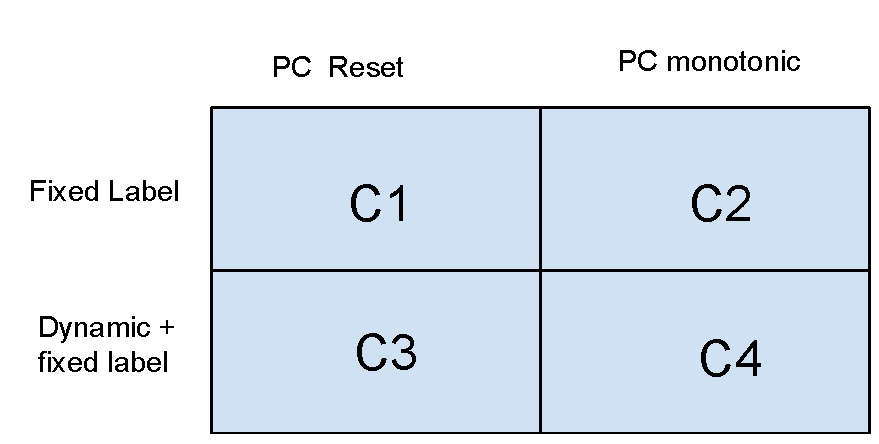
\includegraphics[width=0.6\textwidth]{category}
	\centering
	\caption{Category of constraint generator}
	\label{fig:set}
\end{figure*}
\begin{figure*}[h]
	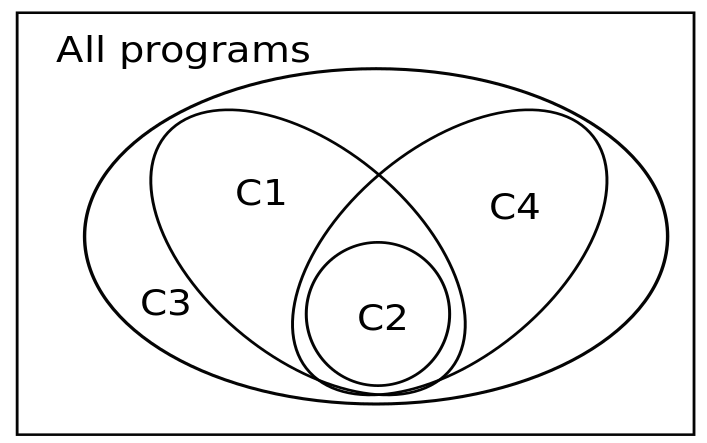
\includegraphics[width=0.6\textwidth]{rsz_set}
	\centering
	\caption{Set diagram}
	\label{fig:set}
\end{figure*}
Figure \ref{fig:set} shows the relationship between set of programs declared secure by all constraint generator. C1-C4 are abbreviation for category 1 - category 4. Number of constraints is inversely proportional to size of set of program declared secure, because more constraints means high probability of violation of security. In category 1 generator generates many false constraints because of absence of dynamic label, but category 3 uses dynamic labels with fixed so it reduces number of constraints. Constraints generated by category 1 are superset of constraints generated by category 3 this relationship shows that set of program declared secure by C1 must be subset of C3. Similarly C2 and C4 differ by use of dynamic labels so set of accepted program by C2 is a subset of set of programs accepted by C4. Use of monotonic PC label helps to capture global information flows so use of monotonic PC label increases the number of constraints. C3 and C4 differ by use of PC label scheme, C4 using monotonic PC and C3 using PC reset so constraints generated by C4 are superset of constraints generated by C3 so set of accepted programs of C4 must be subset of C3. Similarly C2 and C1 differ by PC label scheme so set of accepted programs is a subset of set of programs accepted by C1.    
\begin{figure}
	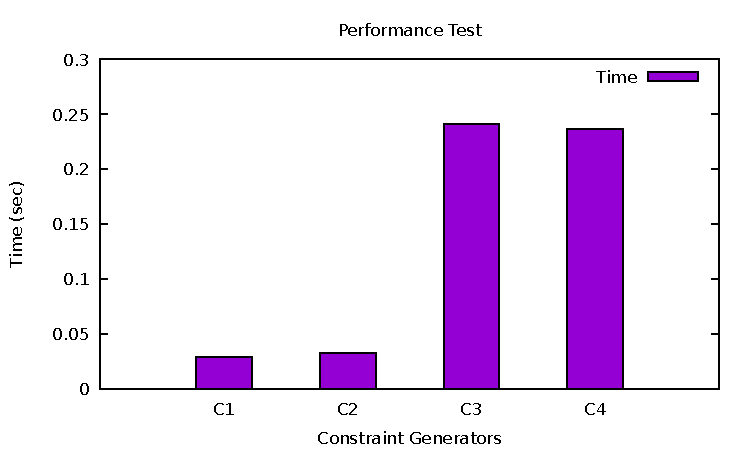
\includegraphics[width=1\textwidth]{graph.pdf}
	\centering
	\caption{Performance test}
	\label{fig:ptest}
\end{figure}
Figure \ref{fig:ptest} shows the average time taken in processing one copy program by all four generator. 
Time taken in order C1 < C2 < C4 < C3. C4 taking little less time than C3 because of optimization in label generation, this optimization uses property of monotonic PC so it can not applied in C3.

\chapter{Implementation of Constraint Generator}
We implemented fully automated certification platform for python source code  using two python scripts, given in Appendix \ref{ch:p1} and \ref{ch:script2}. Block diagram in figure \ref{fig:p1} shows modules of script1, first python source code is converted into abstract syntax tree (AST) with the help of ast library. The purpose of this step is to avoid tedious work of parsing of source code and comments. Figure \ref{fig:parsing} shows that parsing function reads AST word by word. If function finds any desired word it calls other handler functions to handle code related to particular word, for example: if "While" word is found, parsing function parses body of while and passes it as argument to while\_handler(while\_code) function. Handler function parses variables used in condition and passes the body part to parsing function again. Whenever parsing function finds assignment operation it generates constraint and goes to next word.     
\begin{figure}
	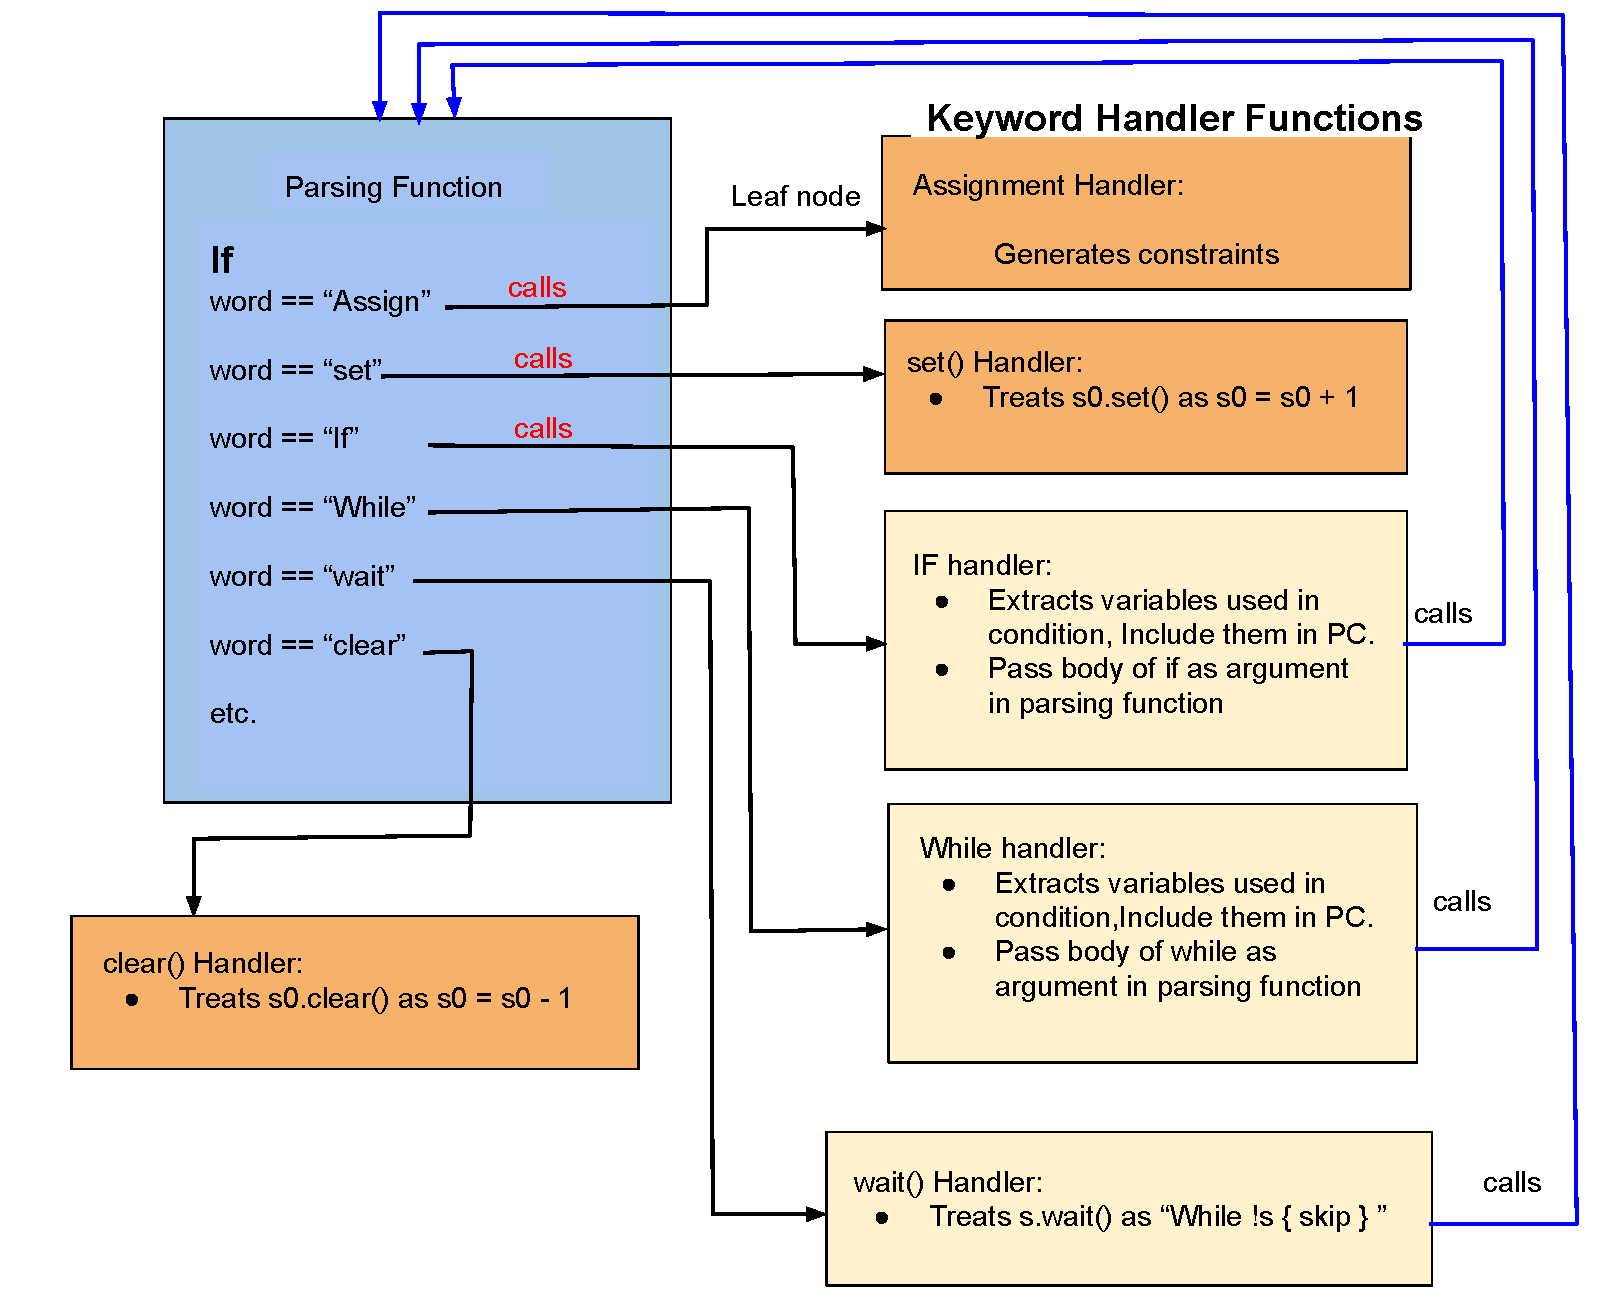
\includegraphics[width=1\textwidth]{parsing.pdf}
	\centering
	\caption{Block diagram of parsing function}
	\label{fig:parsing}
\end{figure}
	The Block diagram for script 2 is given in figure  of chapter . 
	Effectiveness of this platform depends on the phase of constraint generation because if constraint generator fails to track information flow properly then verifier can not produce correct results. Chapter \ref{ch:certify} describe about different constraint generators. Chapter  shows the comparison among all constraint generator.  
	
	\subsection{Contributions}
	\begin{figure}
		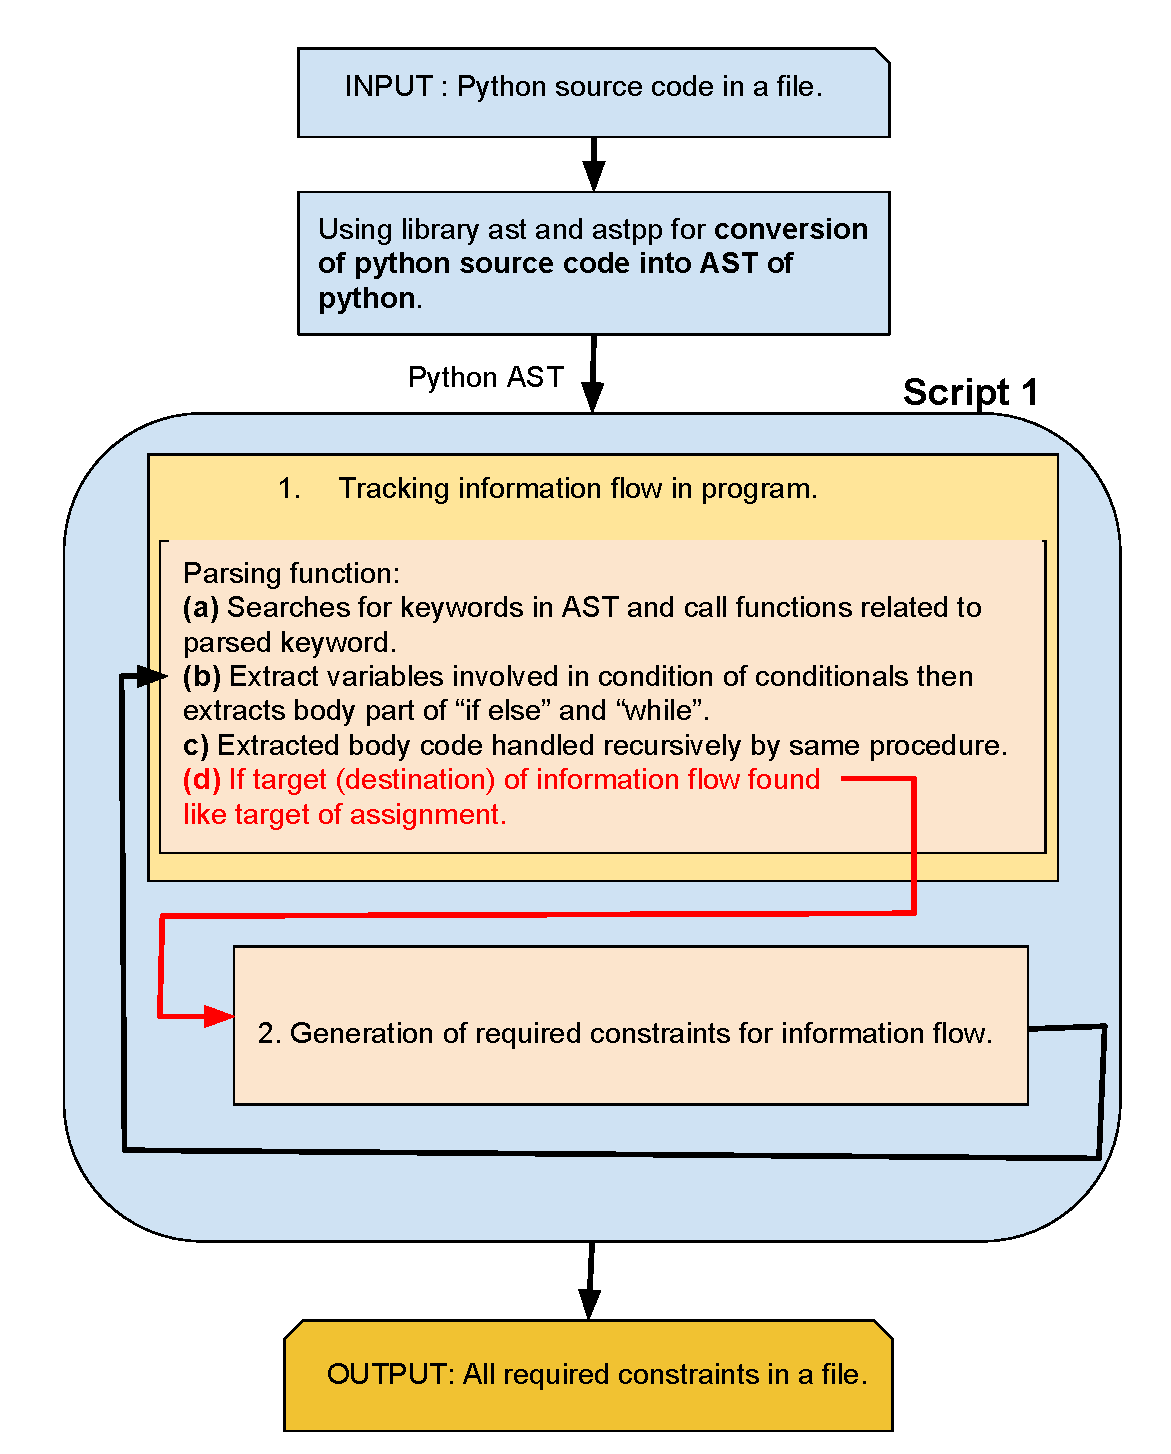
\includegraphics[width=0.6\textwidth]{constraint_gen.pdf}
		\centering
		\caption{Block diagram of script1}
		\label{fig:script1}
	\end{figure}
	Subject considered with objects for certification of python program. Reader Writer Flow Model \cite{rwfm} used to verify information flows in python program.
	\subsection{Implementation Details}
	\textbf{Prerequisite Third Party libraries:}
	\begin{enumerate}
		\item ast python library (for conversion of python source code into abstract syntax tree)
		\item astpp python library (for readability of of abstract syntax tree of python source code)
	\end{enumerate}
	\subsubsection{\textbf{Subset of features of python language considered for analysis.}}
	\begin{itemize}
		\item Assignment operations : x = e (expression)
		\item Conditional statements : "if else", "elif". \item Iteration : "while".
		\item Semaphore operations : set(), wait(), clear(), initialization of semaphore.
		\item Global variables and local variable in a function.
		\item Function calls and definitions.
		\item Return Statement.	 
	\end{itemize}
	
\chapter{Case Study}
\section{Analysis of Multi-threaded Programs}
\label{ch:thread}
In a multi-threaded program, information flows among threads because of communication and synchronization among them. There are two types of semaphores counting and binary, for synchronization among threads. For now, our script handles binary semaphores only. 
\subsection{Handling Information flow due to WAIT and SIGNAL operations}
Traditional operations related to binary semaphore are WAIT and SIGNAL. SIGNAL operation changes the value of semaphore 0 to 1 and WAIT operation wait for an infinite time if the current value of the semaphore is 0 otherwise it changes value 1 to 0 and allows control flow forward. There are three operations related to the binary semaphore in python language wait(), set() and clear(). Traditional WAIT operation can be simulated using python wait() followed by clear() operation, SIGNAL is equivalent to set().\\~\\
\begin{minipage}[b]{0.45\linewidth}
	\centering
	\begin{lstlisting}[ numbers=left, mathescape,%
	caption={Example of wait() operation on binary semaphore.Info Flow: s$\rightarrow$x}, label=lst:wait]
	s = threading.Event()
	s.wait()
	x = 1
	
	\end{lstlisting}
\end{minipage}
\hspace{0.5cm}
\begin{minipage}[b]{0.45\linewidth}
	\centering
	\begin{lstlisting}[ mathescape,%
	caption={Infinite while loop, Information Flow: x$\rightarrow$y }, label=lst:whilewait]
	y = 0
	while x:
	pass
	y = 1
	\end{lstlisting}
\end{minipage}\\
Listing \ref{lst:wait} and Listing \ref{lst:whilewait} show that control flow of wait()  is similar to infinite while loop so we treat wait() in a similar way. All statements which use global variables as a target of assignment and are preceded by wait() may transmit information to other threads. So information flows from semaphore $s_0$ to targets of assignment operations which follows $s_0$.wait() statement.\\
All semaphore operations simplified into normal operations.
\begin{itemize}
	\item s.set() treated as \textbf{s = s + 1}.
	\item s.clear() treated as \textbf{s = s - 1}.
	\item Listing \ref{lst:wait} and \ref{lst:whilewait} shows s.wait() equivalent to \textbf{while(s == 0) \{ skip \}}.
\end{itemize}
\subsubsection{Benchmarking of Certification Script using Denning's Example \cite{denning}}
\begin{lstlisting}[language=Python, caption=Python version of copy3 example in \cite{denning}. goal: information flow from x to y, label={lst:copy3} ]
#Procedure copy3
import thread
import time
import threading
s0 = threading.Event()
s1 = threading.Event()

def thread1():
global x
if x==0:
s0.set()
else:
s1.set()

def thread2():
global y
s0.wait()
s0.clear()
y=1
s1.set()

def thread3():
global y
s1.wait()
s1.clear()
y=0
s0.set()

thread.start_new_thread(thread1,())
thread.start_new_thread(thread2,())
thread.start_new_thread(thread3,())
\end{lstlisting}

To certify the multi-threaded program in Listing \ref{lst:copy3} correctly our script must track information flow from x to y (x $\rightarrow$ y) and must generate constraints accordingly.\\
Constraints generated by our script for program in Listing \ref{lst:copy3} are:
\begin{enumerate}
	\item \dud{x} $\oplus$ \dud{s0} $\leqslant$  \dud{s0}
	\item\dud{x} $\oplus$ \dud{s1} $\leqslant$  \dud{s1}
	\item\dud{s0} $\leqslant$ \dud{s0}
	\item\dud{s0} $\leqslant$ \dud{y}
	\item\dud{s1} $\oplus$ \dud{s0} $\leqslant$  \dud{s1}
	\item\dud{s1} $\leqslant$ \dud{s1}
	\item\dud{s1} $\leqslant$ \dud{y}
	\item\dud{s1} $\oplus$ \dud{s0} $\leqslant$  \dud{s0}
\end{enumerate}  
constraint 1 (\dud{x} $\oplus$ \dud{s0} $\leqslant$  \dud{s0}) and constraint 4 (\dud{s0} $\leqslant$ \dud{y}) \hspace{1cm} $\equiv$ \hspace{1cm} \dud{x} $\leqslant$ \dud{y}.\\
constraint 2 ( \dud{x} $\oplus$ \dud{s1}    $\leqslant$  \dud{s1}) and constraint 7 ( \dud{s1} $\leqslant$ \dud{y}) \hspace{1cm} $\equiv$ \hspace{1cm} 
\dud{x} $\leqslant$ \dud{y}.\\	
Hence script is able to generate correct constraints in multi-threaded program too.


\chapter{Conclusion \& Future work}
\label{ch:conclusion}
We have implemented various algorithms for constraint generation for capturing information flow in program, category 4 algorithm represents intuitive notion of correct security. Second part is verification of constraints using RWFM \cite{rwfm} is also implemented. We considered the subject in information flow analysis, it helps to deal with real world problems related with information flow.\\
\textbf{Future work}
\begin{itemize}
	\item Information flow analysis on python data structures list, dictionary etc.
	\item Information flow analysis related to dynamic types and objects in python
	\item Implementation for all features of python.  
\end{itemize} 


\begin{appendices}
	\chapter{Python Script category 1: Constraint Generator}
	\label{ch:p1}
	\lstinputlisting[language=Python]{p1.py}
	\chapter{Python Script category 2: Constraint Generator}
	\label{ch:p2}
	\lstinputlisting[language=Python]{p2.py}
	\chapter{Python Script category 3: Constraint Generator}
	\label{ch:p3}
	\lstinputlisting[language=Python]{p3.py}
	\chapter{Python Script category 4: Constraint Generator}
	\label{ch:p4}
	\lstinputlisting[language=Python]{p4.py}
	\chapter{Python Script 2: Constraint Checker}
	\label{ch:script2}
	\lstinputlisting[language=Python]{constraint_checker.py}
	\chapter{Copy Programs}
	\label{ch:programs}
	\lstinputlisting[language=Python]{programs.py}
	
\end{appendices}


%\addcontentsline{toc}{chapter}{References}
\bibliography{mylit}
%\bibliographystyle{unsrt}

\end{document}